\documentclass[12pt, twoside]{article}
\usepackage[letterpaper, margin=1in, headsep=0.2in]{geometry}
\setlength{\headheight}{0.6in}
%\usepackage[english]{babel}
\usepackage[utf8]{inputenc}
\usepackage{microtype}
\usepackage{amsmath}
\usepackage{amssymb}
%\usepackage{amsfonts}
\usepackage{siunitx} %units in math. eg 20\milli\meter
\usepackage{yhmath} % for arcs, overparenth command
\usepackage{tikz} %graphics
\usetikzlibrary{quotes, angles}
\usepackage{graphicx} %consider setting \graphicspath{{images/}}
\usepackage{parskip} %no paragraph indent
\usepackage{enumitem}
\usepackage{multicol}
\usepackage{venndiagram}

\usepackage{fancyhdr}
\pagestyle{fancy}
\fancyhf{}
\renewcommand{\headrulewidth}{0pt} % disable the underline of the header
\raggedbottom
\hfuzz=2mm %suppresses overfull box warnings

\usepackage{hyperref}

\fancyhead[LE]{\thepage}
\fancyhead[RO]{\thepage \\ Name: \hspace{4cm} \,\\}
\fancyhead[LO]{BECA / Dr. Huson / Geometry\\*  Unit 7: Congruence transformations\\* 23 January 2023}

\begin{document}

\subsubsection*{7.4 Classwork: Compositions of multiple transformations \hfill CCSS.HSG.CO.A.5}
\begin{enumerate}
\begin{multicols}{2}
  [\item A translation maps triangle $ABC$ onto triangle $DEF$.] \vspace{0.5cm}
    \begin{tikzpicture}[scale=0.9]
      \coordinate [label=above left:$A$](A) at (30:3);
      \coordinate [label=below:$B$](B) at (0, 0);
      \coordinate [label=right:$C$](C) at (-10:3.5);
      \draw [thick] (A)--(B)--(C)--cycle;

      \draw [thick, xshift=4cm, yshift=1.5cm] (30:3) node[above]{$D$}--
      (0,0) node[below]{$E$}--
      (-10:3.5) node[right]{$F$}--cycle;
    \end{tikzpicture}\\
    Fill in the blank with the corresponding object.
    \begin{enumerate}
      \item $A \rightarrow$ \rule{2cm}{0.15mm} \vspace{0.3cm}
      \item $\angle ABC \cong$ \rule{2cm}{0.15mm}
      \item \rule{2cm}{0.15mm} $\cong \overline {EF}$
    \end{enumerate}
  \end{multicols} \vspace{1cm}

\item The vertices of $\triangle JKL$ have the coordinates $J(-4,-2)$, $K(-1,-1)$, and $L(-2,3)$, as shown below. \\[0.5cm]
Apply a translation of $(x,y) \rightarrow (x+7, y+4)$ to $\triangle JKL$ and then reflect the image across the $x$-axis. Draw both images $\triangle J'K'L'$ and $\triangle J''K''L''$ on the set of axes below, labeling the vertices.
\begin{center}
  \begin{tikzpicture}[scale=.48]
    \draw [help lines] (-10,-10) grid (10,10);
    \draw [thick, <->] (-10.4,0) -- (10.4,0) node [right] {$x$};
    \draw [thick, <->] (0,-10.4)--(0,10.4) node [above] {$y$};

    \draw [thick]
    (-4,-2) node[below left] {$J$}--
    (-1,-1) node[right] {$K$}--
    (-2,3) node[above left] {$L$}--
    cycle;
  \end{tikzpicture}\\[0.5cm]
\end{center}

\newpage
\item A rotation of $90^\circ$ is applied to $\triangle ABC$, mapping it onto $\triangle PQR$, as shown.  \\[0.25cm]
Which triangle has the larger area, or are they equal? Justify your answer.\\
  \begin{tikzpicture}[scale=.48]
    \draw [thick, <->] (-7.4,0) -- (10.4,0) node [right] {$x$};
    \draw [thick, <->] (0,-6.4)--(0,10.4) node [above] {$y$};
    \draw [thick]
    (4,-2) node[below left] {$A$}--
    (8,2) node[right] {$B$}--
    (1,1) node[above right] {$C$}--cycle;
    \draw [thick]
    (2,4) node[right] {$P$}--
    (-2,8) node[above] {$Q$}--
    (-1,1) node[below left] {$R$}--cycle;
  \end{tikzpicture}

\item The trapezoid $MATH$, shown below, undergoes two rigid motions carrying it onto trapezoid $COMP$. State the two isometric transformations. (there is more than one correct answer)\\
  \begin{tikzpicture}[scale=.48]
    \draw [help lines] (-10,-10) grid (10,10);
    \draw [thick, <->] (-10.4,0) -- (10.4,0) node [right] {$x$};
    \draw [thick, <->] (0,-10.4)--(0,10.4) node [above] {$y$};
    \draw [thick]
    (-1,-4) node[below left] {$M$}--
    (1,-1) node[above left] {$A$}--
    (4,-1) node[above right] {$T$}--
    (5,-4) node[below left] {$H$}--cycle;
    \draw [thick]
    (0,2) node[below left] {$C$}--
    (-2,5) node[right] {$O$}--
    (-5,5) node[above left] {$M$}--
    (-6,2) node[below left] {$P$}--cycle;
  \end{tikzpicture}

\begin{multicols}{2}
  [\item A rotation of $90^\circ$ around the vertex $B$ of triangle $ABC$ carries it onto triangle $DEF$.] \vspace{0.5cm}
    \begin{tikzpicture}[scale=0.9]
      \coordinate [label=above right:$A$](A) at (30:3);
      \coordinate [label=below:$B$](B) at (0, 0);
      \coordinate [label=right:$C$](C) at (-10:3.5);
      \draw [thick] (A)--(B)--(C)--cycle;
          \draw [fill] (0,0) circle [radius=0.05];
      \draw [thick, rotate=90] (30:3) node[above]{$D$}--
      (0,0) node[left]{$E$}--
      (-10:3.5) node[right]{$F$}--cycle;
    \end{tikzpicture}
    \columnbreak \\
    Fill in the blank with the corresponding object.
    \begin{enumerate}
      \item $A \rightarrow$ \rule{2cm}{0.15mm} \vspace{0.3cm}
      \item $\angle ABC \cong$ \rule{2cm}{0.15mm}  \vspace{0.3cm}
      \item \rule{2cm}{0.15mm} $\cong \overline {EF}$ \vspace{0.3cm}
      %\item Justify that the areas of $\triangle ABC$ and $\triangle DEF$ are equal. Use the words, ``rotation," ``rigid motion," and ``preserves distance." \vspace{2cm}
    \end{enumerate}
  \end{multicols}

\item State the transformation that carries the trapezoid $BECA$, onto $B'E'C'A'$, as shown below. \\
  \begin{tikzpicture}[scale=.48]
    \draw [help lines] (-10,-4) grid (10,8);
    \draw [thick, <->] (-10.4,0) -- (10.4,0) node [right] {$x$};
    \draw [thick, <->] (0,-4.4)--(0,8.4) node [above] {$y$};

    \draw [thick]
    (0,2) node[below right] {$B$}--
    (2,5) node[above left] {$E$}--
    (5,5) node[above right] {$C$}--
    (6,2) node[below left] {$A$}--cycle;

    \draw [thick]
    (0,2) node[below left] {$B'$}--
    (-2,5) node[above right] {$E'$}--
    (-5,5) node[above left] {$C'$}--
    (-6,2) node[below left] {$A'$}--cycle;
  \end{tikzpicture}

Note: For translations, you must state the $x$ and $y$ quantities; for reflections, the line of reflection; for rotations, the center of rotation and quantity in degrees.

\item Find the length of $\overline{AB}$, where $A(5,-6)$ and $B(13,0)$.
    \vspace{4cm}

\newpage
\item The vertices of $\triangle JKL$ have the coordinates $J(-4,-2)$, $K(-5,1)$, and $L(-2,3)$, as shown below. \\[0.5cm]
Apply a translation of $(x,y) \rightarrow (x+6, y-7)$ to $\triangle JKL$ and then reflect the image across the $y$-axis. Draw both images $\triangle J'K'L'$ and $\triangle J''K''L''$ on the set of axes below, labeling the vertices.\\
  \begin{tikzpicture}[scale=.48]
    \draw [help lines] (-10,-10) grid (10,10);
    \draw [thick, <->] (-10.4,0) -- (10.4,0) node [right] {$x$};
    \draw [thick, <->] (0,-10.4)--(0,10.4) node [above] {$y$};

    \draw [thick]
    (-4,-2) node[below left] {$J$}--
    (-5,1) node[above left] {$K$}--
    (-2,3) node[above left] {$L$}--
    cycle;
  \end{tikzpicture}\\[1.5cm]

\item Challenge: Determine relationship of each equation to the line  $y=\frac{4}{3} x-4$, circling either parallel, perpendicular, or neither.
  \begin{enumerate}
    \item $4x-3y=6$ \hspace{1cm} Parallel \qquad Perpendicular \qquad Neither
    \vspace{1.5cm}
    \item $3x+4y=5$ \hspace{1cm} Parallel \qquad Perpendicular \qquad Neither
    \vspace{2.cm}
  \end{enumerate}

\newpage
\item In the diagram below, $\overleftrightarrow{AC}$ has endpoints with coordinates $A(-1,2)$ and $C(9, -3)$.
\begin{center} %4 quadrant regents grid
  \begin{tikzpicture}[scale=.48]
    \draw [help lines] (-7,-5) grid (10,7);
    \draw [thick, <->] (-7.4,0) -- (10.4,0) node [below right] {$x$};
    \draw [thick, <->] (0,-5.4)--(0,7.4) node [left] {$y$};
    \draw [thick] (-1,2)--(9, -3);
    \draw [fill] (-1,2) circle [radius=0.1] node[above left] {$A$};
    \draw [fill] (9, -3) circle [radius=0.1] node[below right] {$C$};
  \end{tikzpicture}
\end{center}
If $B$ is a point on $\overline{AC}$ and $AB {:} BC = 2{:}3$,  what  are  the  coordinates of $B$?



\end{enumerate}
\end{document}